\section{Online Execution}\label{sec:online_execution}
Due to the inevitable disparity between offline synthesis and real-world online terrain conditions, such as variations in terrain shape and position, additional efforts are required to bridge this gap and prevent potential execution failures. The online execution module takes in terrain states $\inpstateterrain \subseteq \inpterrain$ after abstracting the terrain polygons online, a request state $\inpstaterequest \subseteq \inprequest$,
and a strategy $\strategy$
from the offline synthesis module (Sec.~\ref{sec:reactive_gait_synthesis}).
This module then executes the strategy automaton $\strategy$
by solving a MICP problem online again with the actual perceived terrain polygons, potentially different from the ones abstracted offline, 
to generate a reference trajectory for each transition (Sect.~\ref{sec:automaton_online_evaluation}). This reference trajectory 
along with the corresponding contact information will be further tracked by a tracking controller in real time
(Sec.~\ref{sec:tracking_control}).
As shown by the blue lines in Fig.~\ref{fig:combined_offline_online}(c),
if the robot encounters an unseen terrain state, 
% is unexpected and thus not considered by the offline synthesis module,
we leverage online symbolic repair to create new skills that handle the unexpected terrain state and failure transition at runtime 
% $\inpstateterrain$ 
% and re-synthesize a strategy
(Sec.~\ref{sec:online_repair}).
After reaching the request state $\inpstaterequest$,
the robot resets the strategy with a new terrain state, request goal states,
and repeats the execution
until reaching the final goal state.






% During the online execution, we consider the mismatch between the abstracted and continuous information including both the robot and environmental states. 
% The online execution is divided into an online strategy execution process and a tracking control module.

\subsection{Strategy Automaton Execution and Online MICP Modifications}\label{sec:automaton_online_evaluation}
The red path in Fig.~\ref{fig:combined_offline_online}(c) represents the automaton online execution process. Before transitioning to the new symbolic state, an online gait-fixed MICP is solved according to the skill provided by the automaton. The automaton advances only if the MICP successfully finds a solution.
% Algorithm \ref{code:online_automaton} shows the complete steps of performing online evaluation. More specifically, we consider multiple.
% \subsubsection{Online MICP}
Slightly different from the gait-fixed MICP formulation during the offline phase, the online gait-fixed MICP is executed given terrain information from a terrain segmentation module that produces labeled convex polygons.
For example, a skill transitioning from flat terrain to high terrain, as shown in Fig.~\ref{fig:online_micp}(a),  uses  predefined, homogeneous terrain polygons for feasibility check during offline synthesis. Given that, Fig.~\ref{fig:online_micp}(b) illustrates how the  terrain polygons detected online for the same skill may differ from the offline ones in both position and geometry.
\revised{Note that, perception is intentionally treated as out of scope in this paper. We assume an upstream segmentation pipeline (e.g., elevation-mapping with plane segmentation~\citep{miki2022elevation,fankhauser2018robust}) provides labeled convex polygons; in our hardware experiments we use motion-capture-aided manual labeling of polygons, which is sufficient to validate the planning and control framework, although it does not represent a fully autonomous perception stack. Obtaining convex collision-free regions in unstructured environments is non-trivial, and we make no claim that our framework includes a solution to this perception problem. Robust perception integration is left for future work.}
% Since a strategy is already generated offline, the online MICP explicitly knows the chosen gait and the ideal initial and final robot states given by the robot and terrain abstraction.
In addition, the following modifications are highlighted when attempting to transition between two symbolic states in the automaton.
\begin{figure}
    \centering
    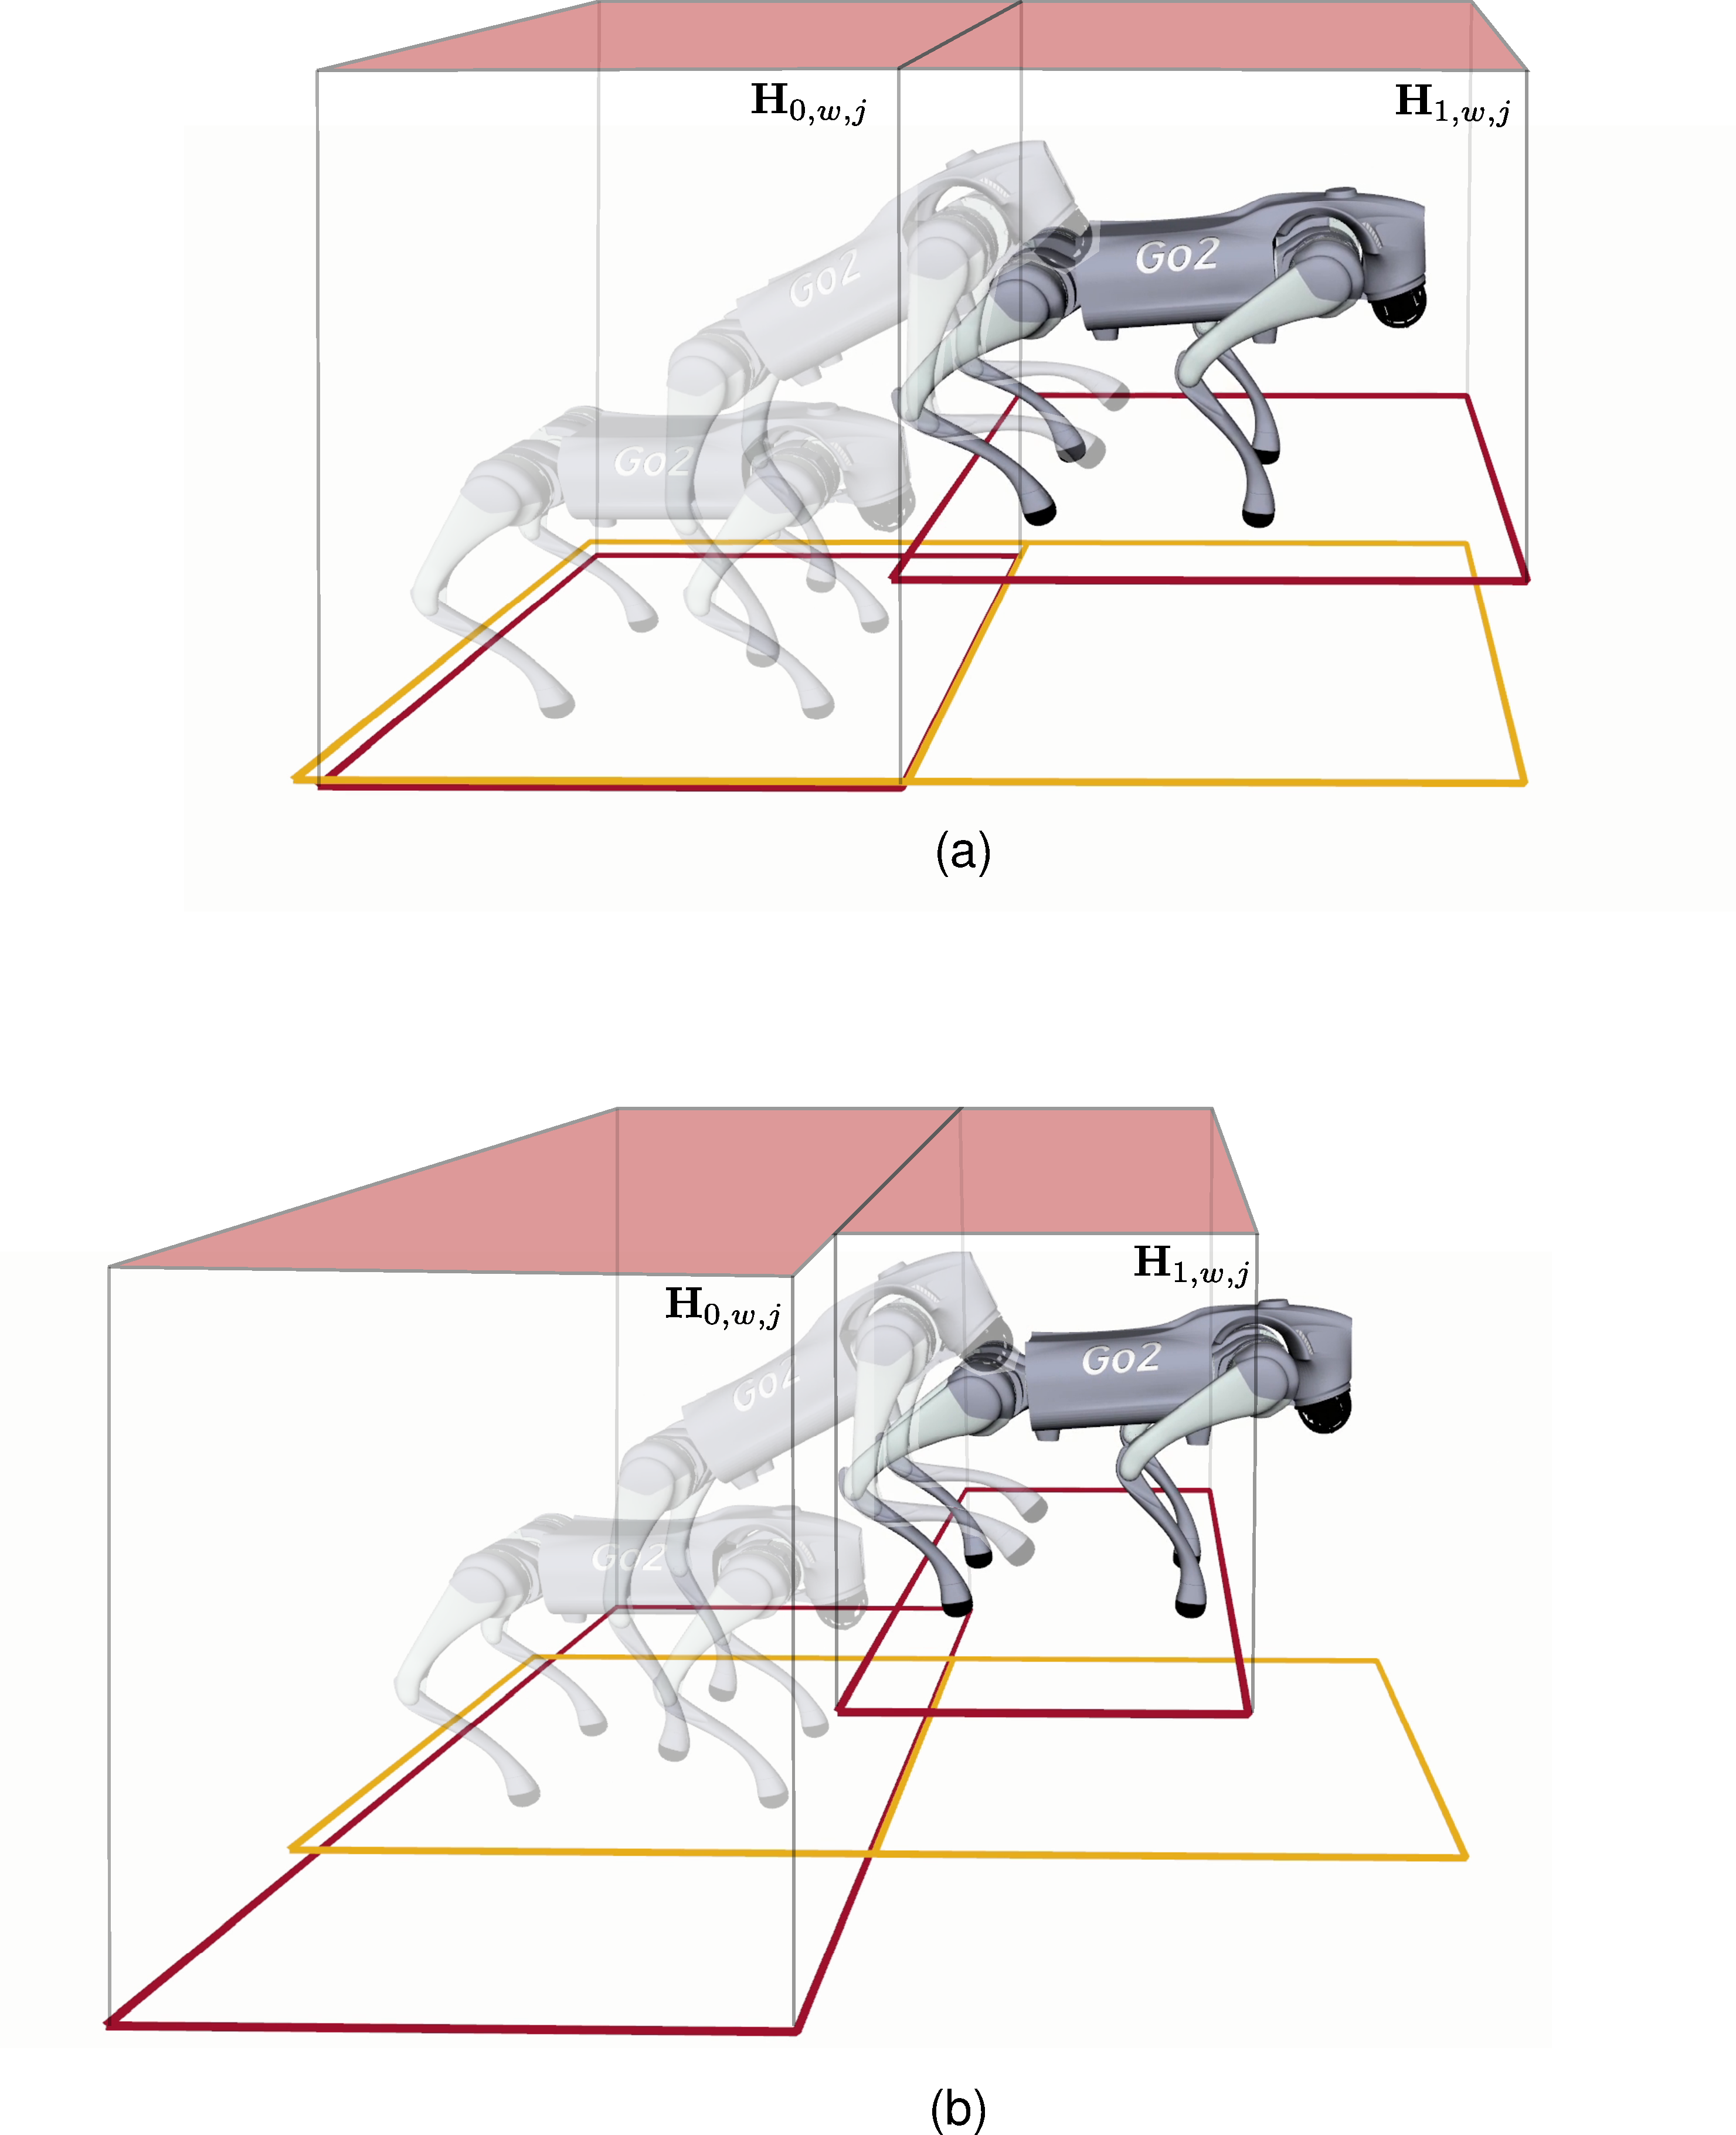
\includegraphics[width=\linewidth]{online_micp.pdf}
    \caption{Demonstrations of (a) offline MICP for a skill transitioning from a flat terrain to a high terrain with predefined polygons; (b) online MICP for the same skill but with online terrain polygons.}
    \label{fig:online_micp}
\end{figure}


\subsubsection{Robot Pose Re-Targeting}
Since the final targeting condition significantly influences the reference trajectory and the feasibility of the MICP problem, we evaluate the final condition by solving a kinematic feasibility problem (a simplified MICP in Eq.~(\ref{ocp:mip_general})) before solving the online MICP. Compared with the gait-fixed MICP, the dynamics equation (\ref{eq:dynamics}) is replaced by enforcing the center of mass (CoM) to lie inside a convex support polygon with all feet in stance to ensure static stability. In addition, a hard constraint is added to ensure that the modified robot pose stays within a certain threshold compared with the original desired pose. The cost function is simplified to stay as close as possible to the original desired pose. The higher-order terms of body position, orientation, and end-effectors are excluded from the decision variables. All the other constraints not involving those higher-order terms remain the same. Once the kinematic feasibility problem is solved successfully, the online MICP is solved using the modified re-targeted final condition and reference trajectory.

\subsubsection{Collision Avoidance and Swing Foot Constraints}
\revised{Our framework handles obstacles at \emph{two distinct levels}, and we will explicitly elaborate which level is responsible in which scenario.
\begin{itemize}
    \item \emph{Symbolic-level obstacle avoidance.} When an obstacle is large enough that an entire abstracted cell becomes unsteppable, it is classified as the \textit{obstacle} terrain class in the local symbolic abstraction (Sec.~\ref{sec:preliminaries_abstraction}). The symbolic specification rules out transitions into such cells, and if an obstacle appears at runtime---as in the rebar-with-obstacle hardware experiment, where the obstacle is detected via motion capture and added to the local abstraction online---runtime symbolic re-synthesis (Sec.~\ref{sec:online_repair}) finds a detour around it. No collision-region variables need to be added to the online MICP in this case.
    \item \emph{MICP-level collision-free region selection (this subsection).} For smaller obstacles that the swing foot must clear within a single symbolic transition, we encode collision avoidance directly in the online MICP. Because the resulting trajectory is sent directly to the tracking controller, the quality of end-effector (EE) trajectories at this layer is critical for tracking performance. We introduce binary variables $\v H_{s,w,j}$ that constrain the swing-foot trajectory of foot $j$ to lie inside one of $S$ pre-labeled collision-free convex polytopes at each time step. These free-space polytopes come from the same labeled-polygon segmentation pipeline as the steppable terrain, with a separate label set distinguishing free-space polytopes from steppable terrain polygons. In simulation, this mechanism is exercised in the \textit{Unstructured--8} case with collision avoidance enabled (see Table~\ref{tab:micp_speed}), where the binary-variable count rises to 256.
\end{itemize}
We do not perform full-body, mesh-level collision checking against arbitrary geometry; the body footprint is implicitly handled by steppable-region selection keeping each foot inside a labeled terrain polygon. The formulation here trades fidelity for online tractability.}

Specifically, $s \in \range{S}$ represents the $s^{\rm th}$ convex collison-free region and $w \in \range{W}$ denotes the $w^{\rm th}$ time step, evenly discretized with $\Delta t_w$ over the entire $W$ time steps. Fig.~\ref{fig:online_micp}(b) demonstrates two collision-free regions.
\begin{align}
    \nonumber & \forall s \in [S], w \in [W], j \in [n_f]\\\label{eq:collision_avoidance} &\v H_{s,w,j} \Rightarrow \v A_s \v p_j[i] \leq \v b_s, \forall i \in \mathcal{C}_{w,w+1}
        \\&\sum_{s=0}^{S-1}\v H_{s,w,j} = 1
        \\&\v H_{s,w,j} \in \{0, 1\}
\end{align}
where $\mathcal{C}_{w,w+1}$ denotes the set of continuous time steps that span from the $w^{\rm th}$ to the ${w+1}^{\rm th}$ binary time step. \revised{We emphasize that the collision-free region selection in Eq.~(\ref{eq:collision_avoidance}) and the steppable-region selection in Eq.~(\ref{eq:safe_region}) handle different geometric primitives: the steppable-region constraint forces \emph{stance-foot} placement onto a labeled steppable terrain polygon at the first stance time step, while the collision-free region constraint here keeps the \emph{swing-foot} trajectory inside a free-space polytope across all time steps within a swing phase. The two are complementary and not redundant.}

To enable larger swing foot clearance from the terrain, we also add constraints to force the swing foot height above a user-defined threshold $h_{\text{swing}}$, given the fixed contact timing. \revised{This constraint targets cleanly clearing the terrain during a transition---for example, when jumping onto a higher platform. While such clearance could in principle be enforced through the collision-free region selection alone, doing so would require a fine time-step discretization of the binary variables and would tend to yield trajectories that only marginally clear the terrain. The height threshold $h_{\text{swing}}$ instead provides a direct, continuously enforced clearance margin that is straightforward to tune.}

\revised{Note that the collision-avoidance and swing-foot constraints are also incorporated in the offline MICP as part of the feasibility-checking rules for the relevant terrain transitions. We highlight them here because their impact on online tracking performance is substantially more critical.}
% \begin{align}
%     &\v p_{j}^z[\text{mid}] \geq \v p_{j}^z[\text{start}] + h_{\text{swing}}\\
%     &\v p_{j}^z[\text{mid}] \geq \v p_{j}^z[\text{end}] + h_{\text{swing}}
% \end{align}
% where $\v p_{j}^z[\text{start}], \v p_{j}^z[\text{mid}], \v p_{j}^z[\text{end}]$ stand for the $j^{\rm th}$ EE positions in the z dimension at the starting, middle, and ending knot point of a swing phase, respectively. 

% \revised{Compared to the conference version~\citep{zhou2025physically}, the binary collision-region variables $\v H_{s,w,j}$, the swing-foot height parameterization, and their joint use in the online MICP are introduced in this article; the underlying gait-fixed MICP structure is shared with the conference version.}

% \begin{algorithm}[h!]\label{code:strategy_execution}
%   \caption{Strategy Execution}
%   \SetAlgoLined
%   \SetKwInOut{Input}{input}\SetKwInOut{Output}{output}
%   \PrintSemicolon
%    \Input{synthesized strategy $\mathcal{A}$, initial robot state $\v x_0$}
%    \Output{referenceTraj, gaitSequence}
%    \nl$\rm curNode$ = initializeNode($\v x_0$)\;
%     \nl\While{1}{
%         \texttt{// Roll out the automaton}\;
%         \nl\If{\rm previousWaypointReached}{
%         \texttt{// Check if local waypoint is changed}\;
%         \nl\If{\rm{!waypointPending} \& \textcolor{blue}{ \rm{localWaypointChanged}}}{
%             setNewWaypoint($\mathcal{X}_{\rm cen}^{\rm des}$, $\rm curNode$, $\mathcal{J}$)\;
%         }
%         \texttt{// Check if local terrain is changed}\;
%         \nl\If{\textcolor{blue}{\rm terrainStateChanged}}{
%             setUpdatedTerrain($\mathcal{E}$, $\rm curNode$, $\mathcal{J}$)\;
%         }
%         \texttt{// Find the next node and solve OCP}\;
%         \nl$\rm{nextNode}$ = findNextAllowableNode($\rm curNode$, $\mathcal{J}$)\;
%         \texttt{// Check goal pose feasibility}\;
%         \nl$\v x_{\rm init}$ = $\rm{referenceTraj}[-1]$\;
%         \nl($\rm goalFeasible$, $\v x_{\rm goal}$) = \textcolor{blue}{ solveInstantaneousOCP}($\rm nextNode$)\;
%         \nl\eIf{\rm goalFeasible}
%         {
%             \nl($\rm OCPsuccess$, $\rm traj$, $\rm gait$) = \textcolor{blue}{solveOCP($\rm curNode$, $\rm nextNode$)\;}}
%         {
%             \nl \textcolor{blue}{triggerReplan}\;
%         }
        
%         \nl\eIf{\rm OCPsuccess}{
%             \nl$\rm referenceTraj$ += $\rm traj$\;
%             \nl$\rm gaitSequence$ += $\rm gait$\;
%         }{
%             \nl \textcolor{blue}{triggerReplan}\;
%         }
%         \texttt{// Publish reference trajectory and gait}\;
%         \nl\If{$\mathcal{X}_{\rm cen} = \mathcal{X}_{\rm cen}^{\rm des}$}{
%             \nl publishReference($\rm referenceTraj$, $\rm gaitSequence$)\;
%             \nl clearReferenceTrajAndGait()\;
%             \nl \textcolor{blue}{requestReset}\;
%         }
%         \nl$\rm curNode$ = $\rm nextNode$\;
%         }
%         $\texttt{// Reset the current node}$\;
%         \nl\If{\rm resetRequested \& \rm{goalReached}} {
%             \nl$\rm curNode$ = findNodeAfterReset($\mathcal{E}$, $\rm curNode$, $\mathcal{J}$)\;
%         }
%     }
% \end{algorithm}

% \subsection{Online Repair}\label{sec:online_repair}
% During online execution, 
% the robot may encounter unexpected terrain states
% that the initial model of the workspace structure does not take into consideration.
% We leverage an online repair tool~\citep{meng2024automated} 
% to detect and recover from such unexpected terrain states.

% The online repair tool first generates a monitor that detects violations of the environment assumptions $\envsafety$ during online execution.
% %
% Note that $\envsafety$ includes the assumption
% $\envterrain = $ $
%     \square (
%     \bigvee_{\statevar\in\inpstateterrainposs}
%     \form{\inpterrain}{\statevar})$,
% which assumes that 
% at any time, 
% at least one terrain state from the set of possible terrain states $\inpstateterrainposs$ must hold
% % the current terrain state $\inpstateterrain$
% % must always come from
% % $\inpstateterrainposs$, 
% % the set of possible terrain states provided by the user
% (see Sec.~\ref{sec:spec_gen}).
% % Suppose the current terrain state $\inpstateterrain$ is not in $\inpstateterrainposs$, the set of possible terrain states provided by the user.
% During online execution,
% if the current terrain state $\inpstateterrain \not\in \inpstateterrainposs$,
% the monitor detects that $\inpstateterrain$
% violates the assumption $\envterrain$.
% We then relax the violated assumption $\envterrain$ to admit the new terrain state $\inpstateterrain$,
% replacing $\envterrain$ with 
% $\square (
%     \bigvee_{\statevar\in\inpstateterrainposs\cup\{\inpstateterrain\}}
%     \form{\inpterrain}{\statevar})$.
% After assumption relaxation,
% the revised specification becomes unrealizable
% as the robot lacks the required skills to handle the new terrain state $\inpstateterrain$.
% We utilize symbolic repair 
% (Sec.~\ref{sec:symbolic_repair})
% to find a set of necessary skills for the new terrain state.
\subsection{Runtime Repair}\label{sec:online_repair}
% The runtime repair takes in
% a terrain state $\inpstateterrain \in \inpstatesterrain$, 
% a request state $\inpstaterequest \in \inpstatesrequest$,
% and a Boolean formula $\disallowedtrans$
% representing disallowed transitions discovered at runtime.
% We first update the system hard constraint $\syssafety$ in the specification $\spec$ from Sec.~\ref{sec:spec_gen}
% to be $\syssafety \land \square \disallowedtrans$,
% so that the updated specification respects the newly discovered disallowed transitions, if any.
% We then
% leverage the high-level manager to create a partial evaluation of $\spec$ over $\inpstateterrain$ and $\inpstaterequest$,
% and perform symbolic repair 
% to generate new robot skills and a new strategy to handle $\inpstateterrain$ and $\inpstaterequest$,
% as done in Sec.~\ref{sec:manager_and_repair}.
The runtime repair procedure takes as input a terrain state $\inpstateterrain \in \inpstatesterrain$, a request state $\inpstaterequest \in \inpstatesrequest$, and a Boolean formula $\disallowedtrans$ that encodes disallowed transitions identified at runtime. We first update the system’s hard constraint $\syssafety$ in the specification $\spec$ (see Sec.~\ref{sec:spec_gen}) to $\syssafety \land \square \disallowedtrans$, ensuring that the specification reflects these newly discovered restrictions. Next, the high-level manager constructs a partial evaluation of $\spec$ over $\inpstateterrain$ and $\inpstaterequest$. Symbolic repair is then applied to generate additional robot skills and synthesize a new strategy that accommodates the current terrain and request states, following the approach in Sec.~\ref{sec:manager_and_repair}.





% the prior knowledge of the workspace structure does not take into account.
% \begin{enumerate}
%     \item Encounter unexpected terrain states during execution
%     \item Generate a monitor to check assumption violations
%     \item The monitor detects that the new terrain state violates the environment assumption which states that the current terrain state must belong to the set of possible terrain states.
%     \item we relax the assumption to include the new terrain state
%     \item we perform repair obtain new skills that can handle the new terrain state, and resume the execution
% \end{enumerate}


\section{Tracking Control}\label{sec:tracking_control}
The tracking control module adopts an MPC-Whole-Body-Control (WBC) hierarchy, ensuring precise end-effector (EE) and centroidal momentum tracking. To smoothly and efficiently execute the strategy considering the potential computational delay in solving MICP, a harmonic coordination module between the strategy automaton roll-out and the tracking module is designed (Sec.~\ref{sec:coordination}).

\subsection{Tracking Control Module}
\subsubsection{Nonlinear Model Predictive Control (NMPC)}\label{subsec:nmpc}
The NMPC  operates independently from the symbolic planning module, tracking reference trajectories generated by the online MICP using a more accurate dynamics model. In this work, the NMPC accounts for the robot's centroidal dynamics and kinematics, similar to approaches in \citep{dai2014whole,chignoli2021humanoid,sleiman2021unified}, presenting a more accurate model than the simplified angular dynamics in the MICP. An analytical inverse kinematics solution based on the MICP output provides the full joint state reference trajectory for the NMPC.
In addition to standard frictional and contact constraints and base tracking costs, an additional cost function for EE reference tracking from the MICP is included to enhance precision. The NMPC optimization problem is formulated as a Sequential Quadratic Program (SQP) and solved using the OCS2 library \citep{OCS2}, with a time horizon of one second and 100 knot points.

\subsubsection{Whole-Body Control (WBC)}
While NMPC operates at the centroidal level to generate dynamically feasible trajectories, WBC ensures precise execution by resolving full-body state control, including joint torques, accelerations, and contact forces.
The whole-body controller tracks the NMPC trajectory by solving a weighted quadratic program (QP) \citep{kuindersma2014efficiently} at 500 Hz. To improve the performance of agile motions such as leaping and jumping, centroidal momentum tracking \citep{wensing2013generation} is included. This MPC-WBC hierarchy allows the system to handle both centroidal-dynamics-level and full-body-dynamics-level control in a coordinated manner, ensuring robustness in real-world deployment especially for highly dynamic motions such as jumping.

\subsubsection{State Estimation}
The state estimator employs a linear Kalman filter similar to that in \citep{bledt2018cheetah}, with the addition of OptiTrack motion capture (mocap) measurements fused alongside IMU data and joint encoder readings to achieve accurate body position estimation. For agile motions such as jumping, we observed improved base-height estimation by assigning higher noise values to the mocap feedback during aerial phases, due to its limited 120 Hz update rate.
\subsection{Coordination between Strategy Execution and Tracking Module}\label{sec:coordination}
\begin{figure}
    \centering 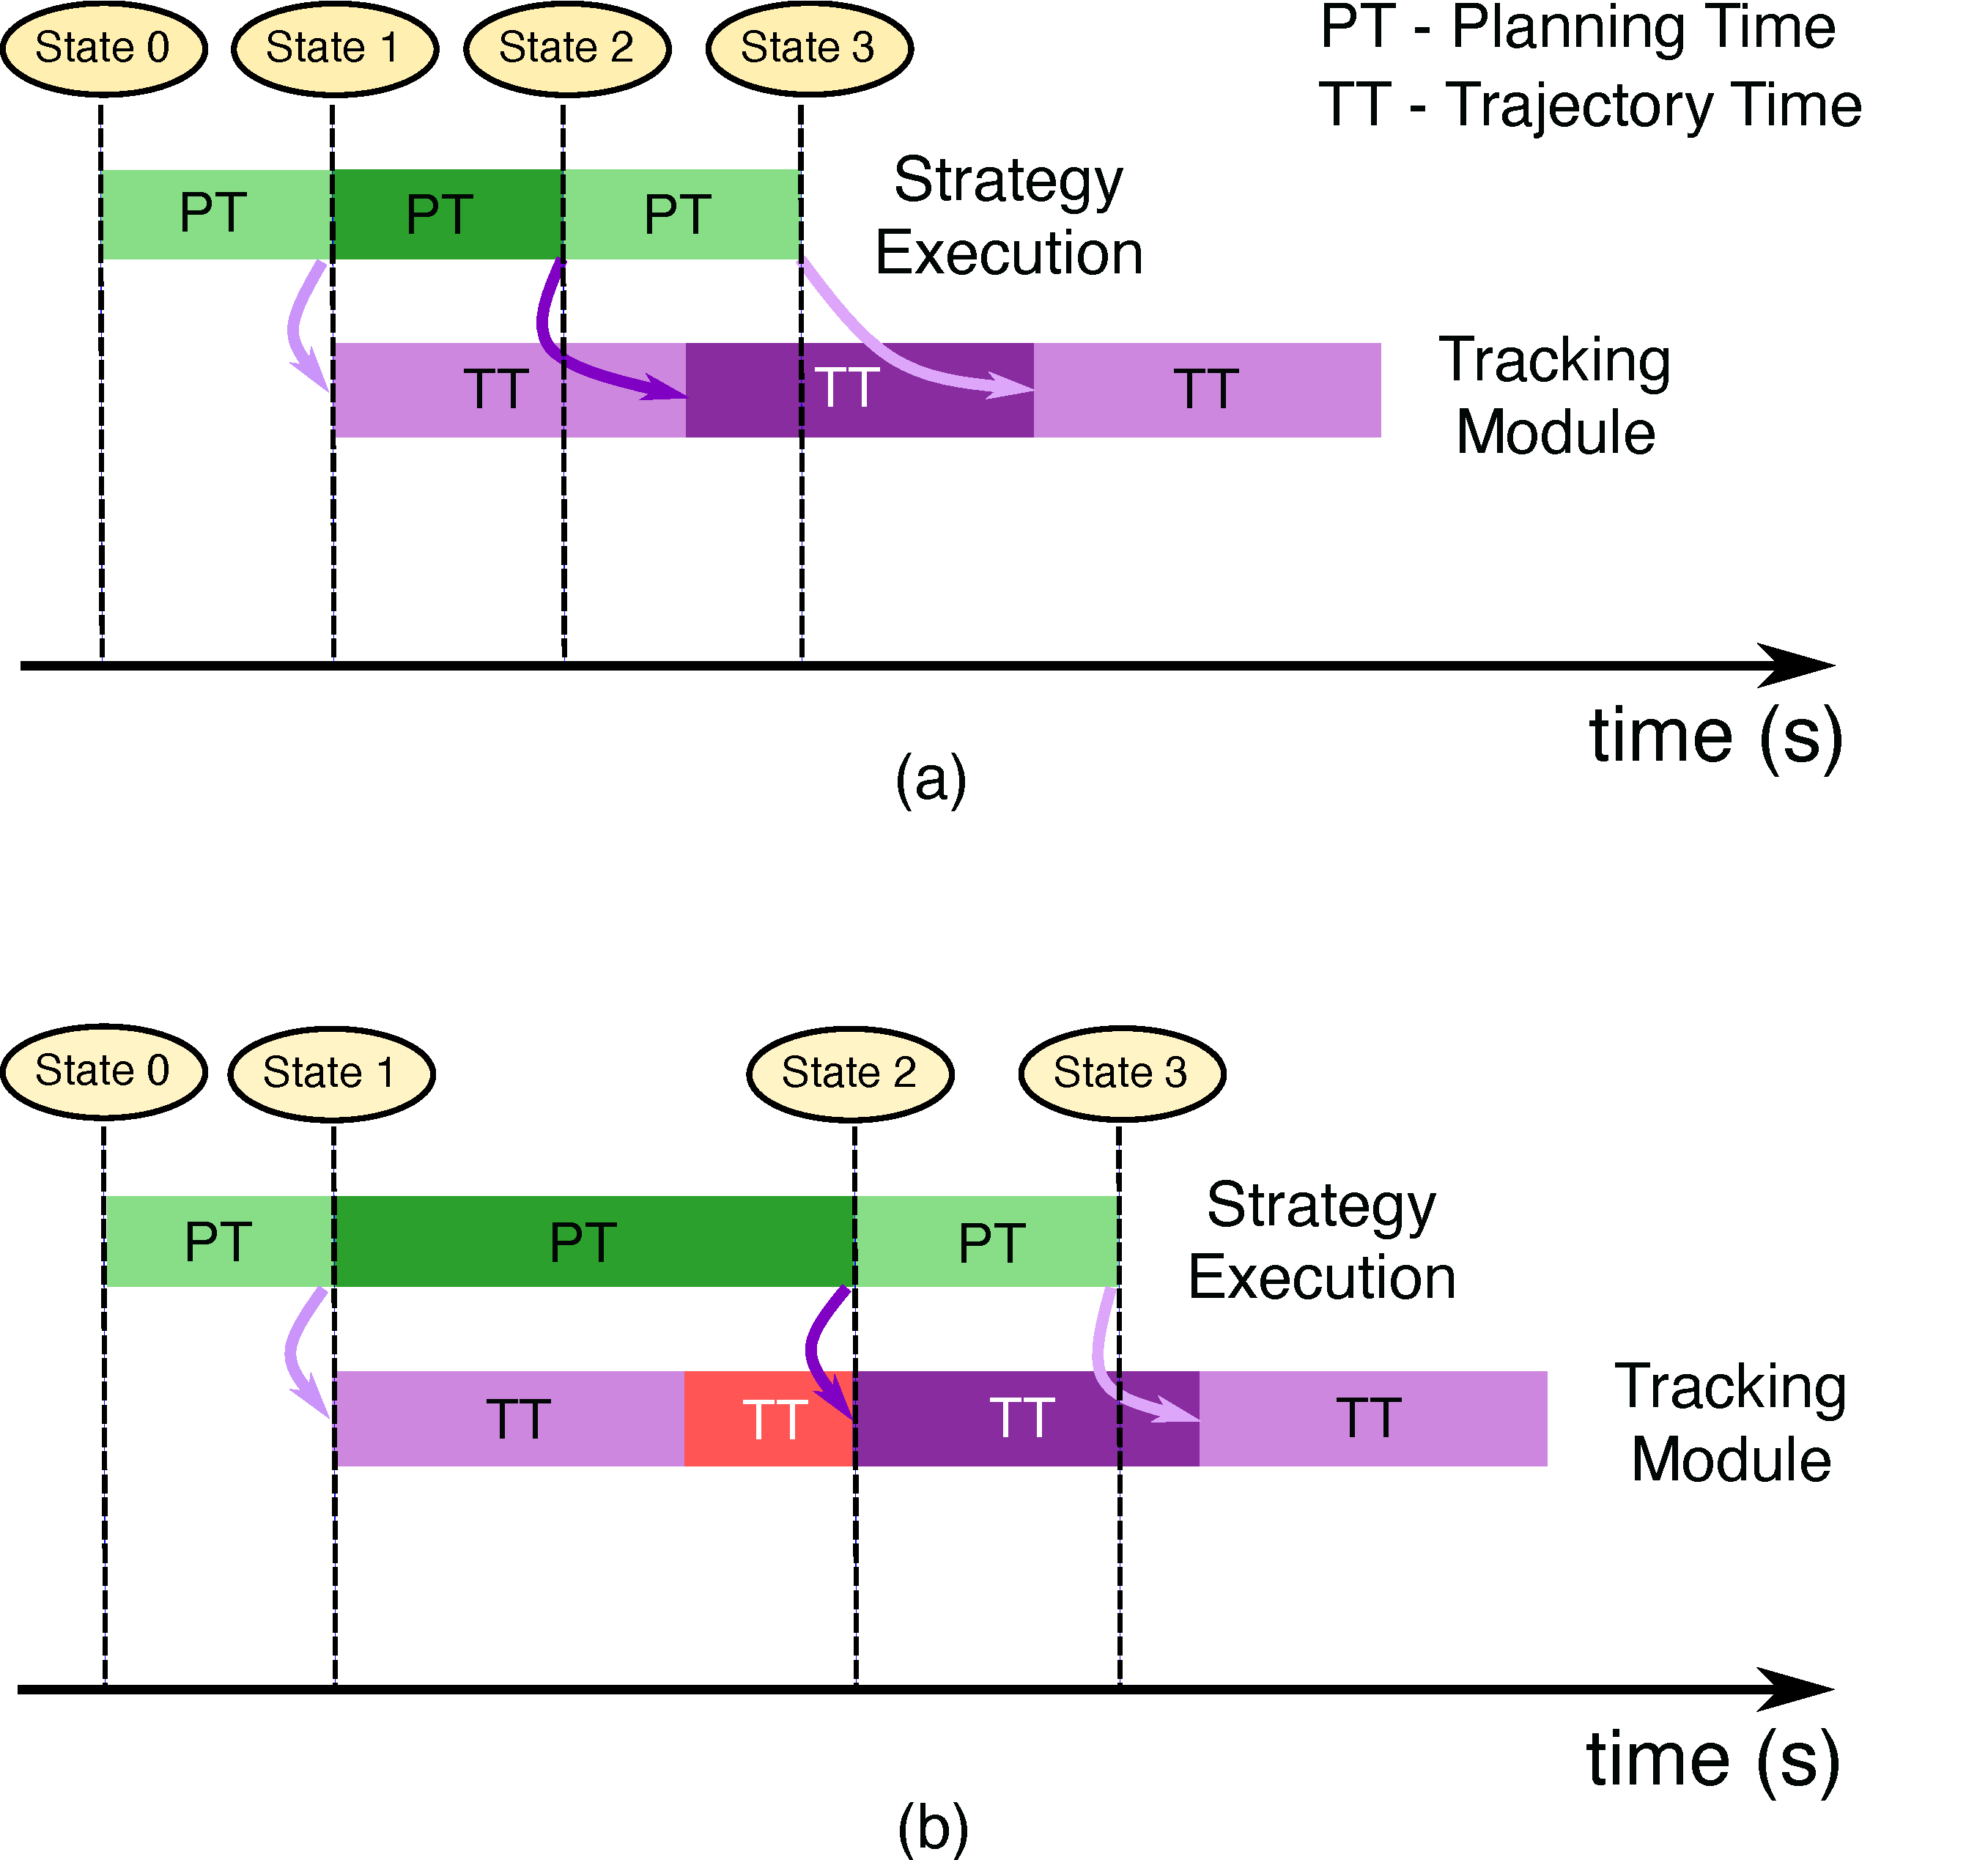
\includegraphics[width=\linewidth]{multi_threading_new.pdf}
    \caption{Coordination between strategy execution and tracking control module.
    (a) The MICP solving time (denoted by PT) for transitioning from State 1 to State 2 is shorter than the time horizon of the previous reference trajectory (denoted by TT), allowing the seamless appending for the new trajectory.
    (b) The MICP solving time exceeds the time horizon of the previous reference trajectory, requiring the robot to come to a stop (red) and wait for the new trajectory whenever available.}
    \label{fig:micp_mpc_automaton}
\end{figure}
Due to the potential delays in solving MICP during the strategy automaton roll-out, a harmonic coordination between the strategy execution and tracking control module is essential. The tracking module's reference trajectory is updated dynamically alongside the strategy execution process, as shown in Fig.~\ref{fig:micp_mpc_automaton}. The overall process can be summarized as follows:

\subsubsection{Strategy Execution} The strategy automaton execution thread begins by solving the online gait-fixed MICP, starting from State 0 in the automaton. Once the MICP solution is obtained, it immediately sends the reference trajectories and corresponding contact information to the tracking control module. The automaton then progresses to the next transition, using the final condition in the previous trajectory segment as the new initial condition. In Fig.~\ref{fig:micp_mpc_automaton}, the colored blocks in the strategy execution timeline indicate the time taken for each MICP solve during the automaton roll-out. PT and TT denote the planning time and trajectory time, respectively.

\subsubsection{Tracking Control Module}
The MPC-WBC tracking control module receives time-indexed reference trajectories, which can be updated in real-time. After completing the tracking of the current reference trajectory, the robot returns to a stance phase, ready to accept new reference trajectories. As depicted in Fig.~\ref{fig:micp_mpc_automaton}, the colored blocks in the tracking control module represent the time horizon of each reference trajectory sent by the strategy execution thread. Once the initial reference trajectory is generated, the MPC-WBC thread begins tracking it using more accurate dynamics models, as described in Sec.\ref{sec:tracking_control}.

\subsubsection{Delay Handling}
For more complex scenarios involving a larger number of terrain polygons, the MICP solving time may increase and exceed the time horizon of the generated reference trajectory. Fig.~\ref{fig:micp_mpc_automaton}(a) and (b) illustrate two cases of MICP solving times:
Case (a): The solving time for transitioning from automaton State 1 to State 2 is shorter than the time horizon of the previous reference trajectory. In this case, the new reference trajectory is seamlessly appended to the existing one, and the robot continues tracking the previous trajectory.
Case (b): The solving time exceeds the time horizon of the previous reference trajectory, and the robot has already entered a stance phase (red block) when the MICP solution is obtained. In this case, the robot waits until the newly generated reference trajectory is sent based on the current system time (red block in Fig.~\ref{fig:micp_mpc_automaton} (b)).

% \subsubsection{Error Handling and Replanning}
% If the MPC thread predicts a state that reaches the final state but deviates beyond the specified tolerance, the automaton thread resets to this new initial state and reruns the MICP to adjust the plan. If no significant deviation occurs, the automaton thread continues rolling out, using the desired state until the local waypoint is reached.

